The warm interface electronics must provide an interface between the Cold Electronics and DAQ, timing and slow control systems, including local power control at the flange and a real-time diagnostic readout. They are housed in the WIECs attached directly to the CE flange.  The WIEC shown in Figure~\ref{fig:tpcelec-flange} 
contains one
Power and Timing Card (PTC), five Warm Interface Boards (WIBs) and a passive
Power and Timing Backplane (PTB), which fans out signals and LV power from the PTC to the WIBs. The WIEC must provide a Faraday-shielded housing, robust ground connections from the warm electronics boards to the detector ground described in Section~\ref{DETECTOR GROUND}, and only optical fiber links to the DAQ and slow control, to mitigate noise introduced at the CE feed-through.

\begin{dunefigure}
[Exploded view of the CE signal flange for ProtoDUNE-SP.  The design will be very similar for the DUNE far detector CE signal flange (with two CE signal flanges per feed-through).]
{fig:tpcelec-flange}
{Exploded view of the CE signal flange for ProtoDUNE-SP.  The design will be very similar for the DUNE far detector CE signal flange (with two CE signal flanges per feed-through).}
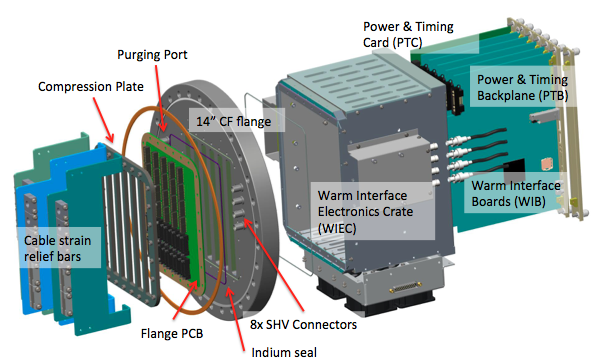
\includegraphics[width=0.9\linewidth]{tpcelec-flange.png}
\end{dunefigure}

The WIB is the interface between the
DAQ system and four
FEMBs. It receives the system clock and control signals from the
timing system and provides for processing and fan-out of those signals to the four
FEMBs. The WIB also receives the high-speed data signals from the four 
FEMBs and transmits them to the DAQ system over optical
fibers. The data signals are recovered onboard the WIB with commercial equalizers.
The WIBs are attached directly to the TPC
CE feedthrough on the signal flange. The feedthrough
board is a PCB with connectors to the cold signal and LV power cables fitted
between the compression plate on the cold side, and sockets for
the WIB on the warm side. Cable strain relief for the cold cables is 
supported from the back end of the feedthrough.

\begin{dunefigure}
[Power and Timing Card (PTC) and timing distribution to the WIB and FEMBs used in ProtoDUNE-SP.]
{fig:tpcelec-wib_timing}
{Power and Timing Card (PTC) and timing distribution to the WIB and FEMBs used in ProtoDUNE-SP.}
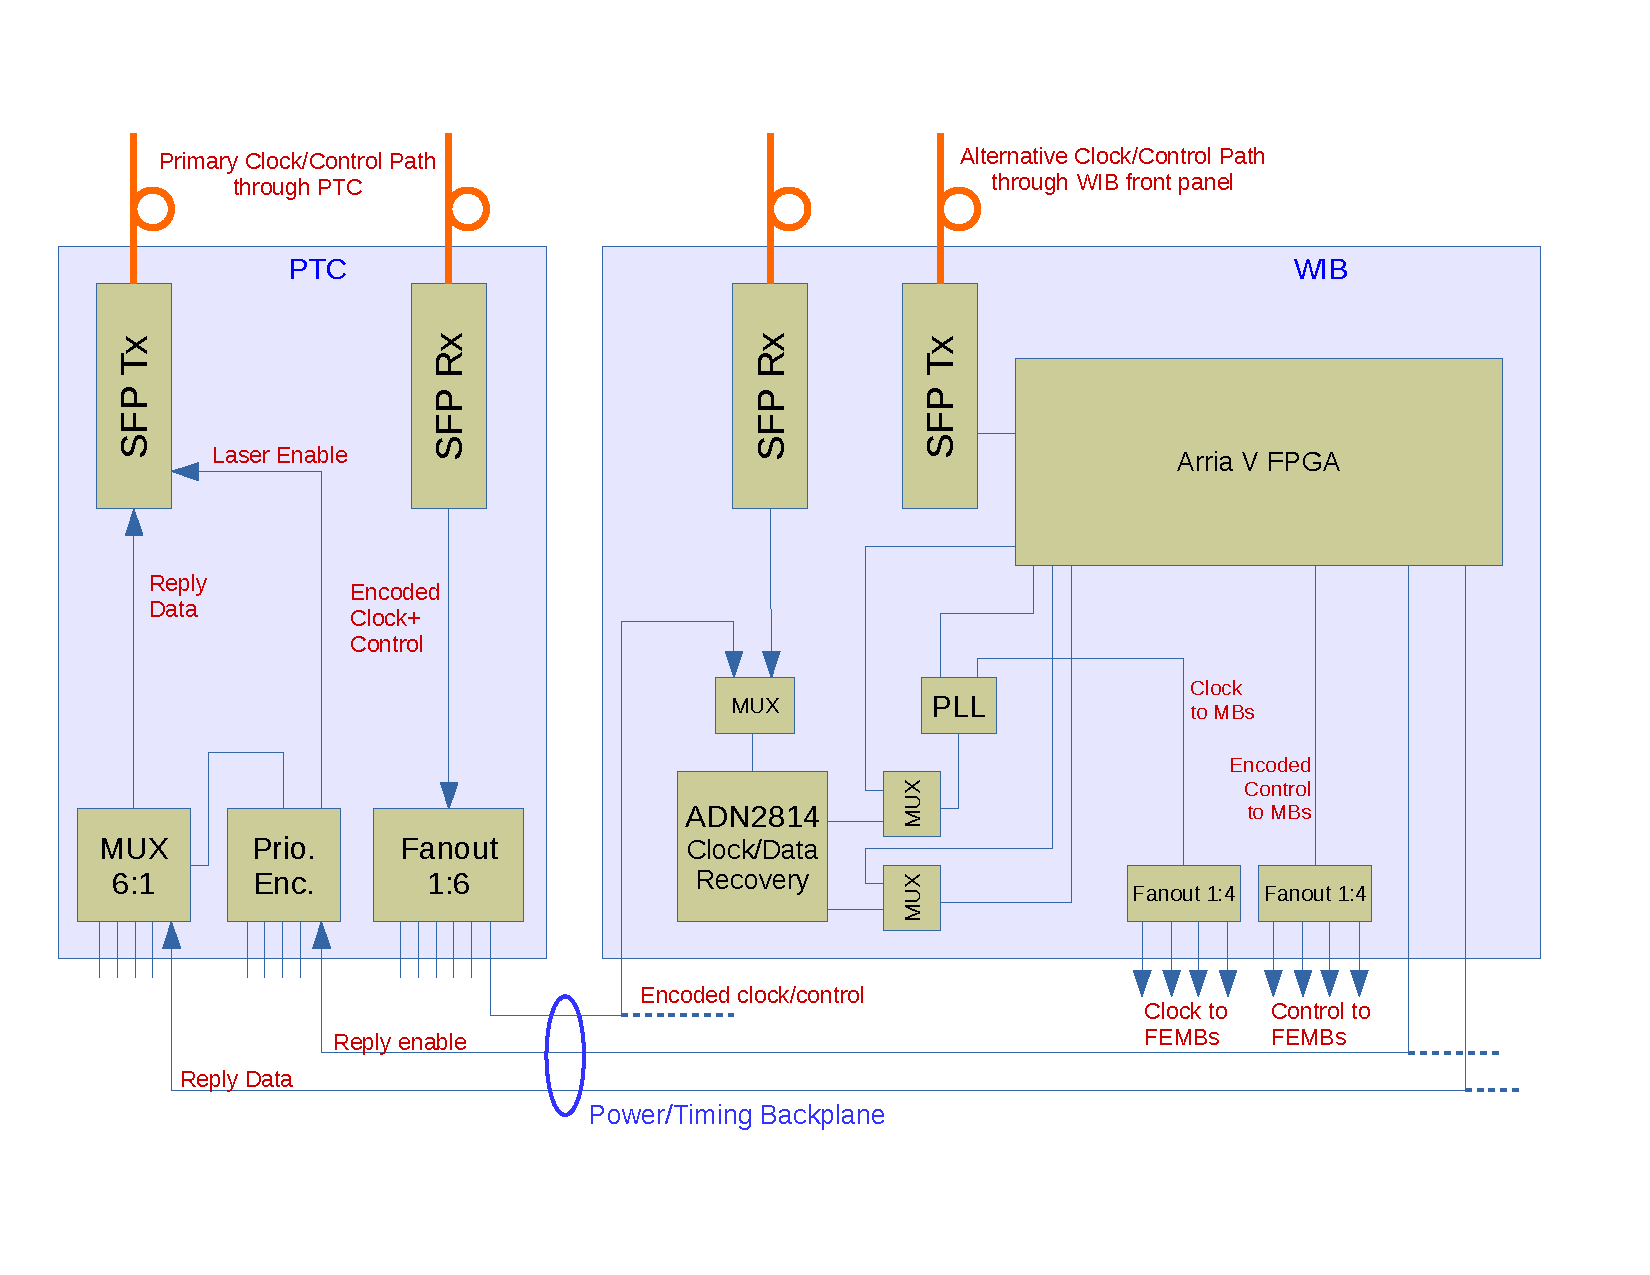
\includegraphics[width=0.8\linewidth]{tpcelec-wib_timing.pdf}
\end{dunefigure}

The ProtoDUNE-SP PTC provides a bidirectional fiber interface to the
timing system. The clock and data
streams are separately fanned-out to the five WIBs as shown in
Figure~\ref{fig:tpcelec-wib_timing}. The PTC fans the clocks out to the WIB over the
PTB, which is a passive backplane attached directly to the PTC and
WIBs.  The received clock on the WIB is separated into clock and
data using a clock/data separator. Timing endpoint firmware to receive and transmit
the clock is integrated in the WIB FPGA (the Altera Arria V was used for ProtoDUNE-SP).
The single-phase far detector timing system, described in~\ref{sec:fdsp-daq-timing}, is a development of the ProtoDUNE-SP system, and expected to require the nearly identical functionality at the WIB endpoint.

\begin{dunefigure}
[LV power distribution to the WIB and FEMBs implemented for ProtoDUNE-SP. This will be modified for DUNE to provide the required voltage or voltages depending on which ASICs are used on the FEMBs. In particular the voltages to the FEMB0-3 will change as the ProtoDUNE-SP FPGA is replaced by COLDATA. ]
{fig:tpcelec-wib_power}
{LV power distribution to the WIB and FEMBs implemented for ProtoDUNE-SP. This will be modified for DUNE to provide the required voltage or voltages depending on which ASICs are used on the FEMBs. In particular the voltages to the FEMB0-3 will change as the ProtoDUNE-SP FPGA is replaced by COLDATA. }
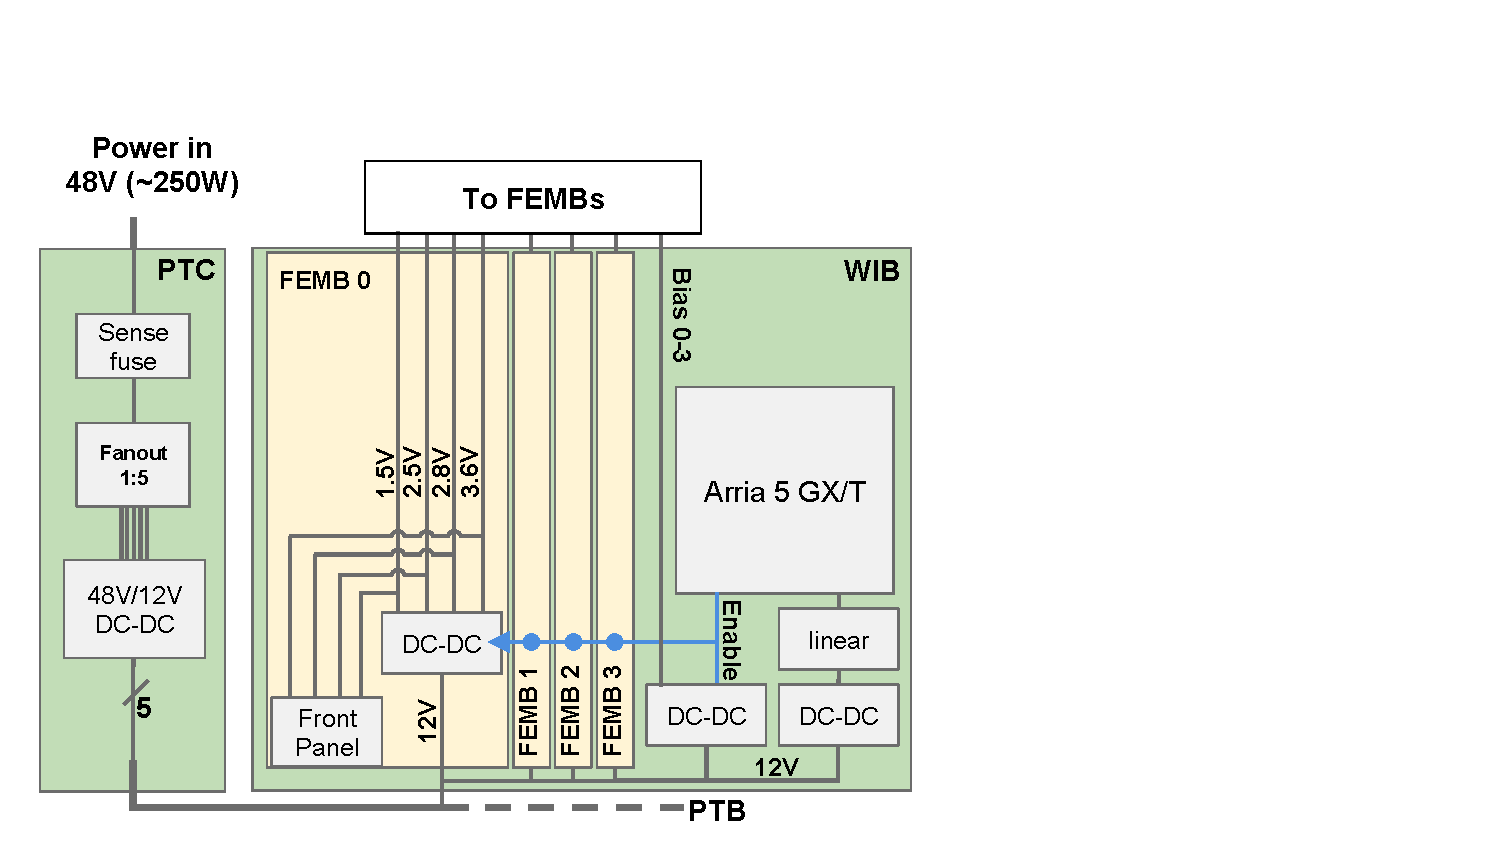
\includegraphics[width=0.7\linewidth]{tpcelec-wib_power.pdf}
\end{dunefigure}

The PTC also receives 48V LV power for all cold
electronics connected through the TPC signal flange: one~PTC, five~WIB, and 20~FEMB. The LV power is then stepped down
to 12V via a DC/DC converter onboard the PTC. The output of the PTC converters is filtered with a common-mode choke and fanned out
on the PTB to each WIB, which provides the necessary 12V DC/DC conversions and fans
the LV power out to each of the cold FEMBs supplied by that WIB, 
as shown in Figure~\ref{fig:tpcelec-wib_power}. The output of the WIB converters are further filtered by a common-mode choke. The 
majority of the power drawn by a full flange is dissipated in the LAr by the cold FEMB.

%Each WIB contains a 
%unique IP address for its UDP slow control interface. The IP address for the WIB is 
%derived from a crate and slot address: the crate address is generated on the PTC 
%board via dipswitches and the slot address is generated by the PTB slot, numbered 
%from one to five. Note that the WIBs also have front-panel
%connectors for receiving LV power; these can be used in place of 
%the LV power inputs on the PTB generated by the PTC.

As shown in Figure~\ref{fig:tpcelec-dune_wib}, the WIB is capable of receiving LV power in the front panel and distributing it directly to the FEMB, bypassing all DC/DC converters.
It can also receive the encoded system timing signals over bi-directional optical
fibers on the front panel, and processing these using either
the on-board FPGA or clock synthesizer chip to provide the clock required by the cold electronics.
The baseline ASIC design currently uses 8b/10b encoding; if the SLAC CRYO ASIC is selected for
the detector's construction, 12b/14b encoding will be used instead of 8b/10b.

\begin{dunefigure}
[Warm Interface Board (WIB). Note that front panel inputs include a LEMO connector and alternate inputs for LV power and timing.]
{fig:tpcelec-dune_wib}
{Warm Interface Board (WIB). Note that front panel inputs include a LEMO connector and alternate inputs for LV power and timing.}
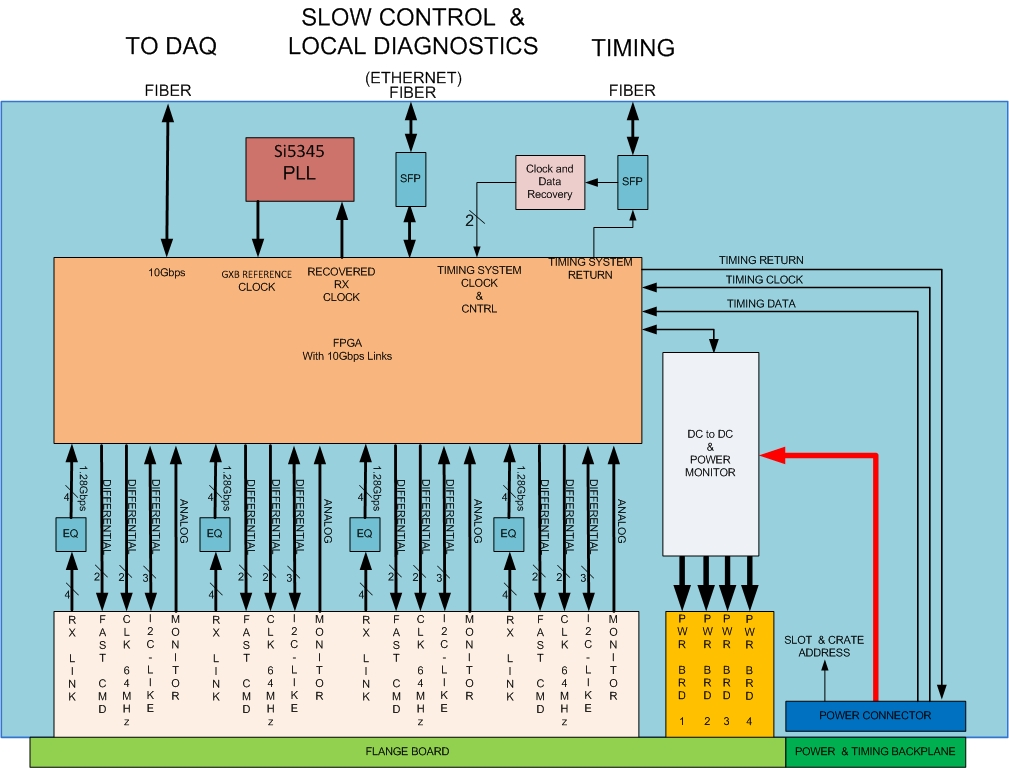
\includegraphics[width=0.9\linewidth]{tpcelec-dune_wib.jpg}
\end{dunefigure}

The FPGA on the ProtoDUNE-SP WIB is an Altera Arria V GT variant, which has
transceivers that can drive the high-speed data to the DAQ system up to
10.3125~Gbps per link, implying that all data from
two FEMB (2$\times$5~Gbps) could be transmitted on a single link.
The FPGA has an additional Gbps Ethernet transceiver I/O based on the 125~MHz clock, which 
provides real-time digital data readout to the slow control system.
